\subsection{Sum of Processed Samples}

The sum of processed samples has been generated by a query to the database (see \autoref{lst:sqlprocessedsamples}) of the \ac{DoHG@MHH}'s \ac{LIMS}.

\begin{table}[H]
\centering
\caption{Sum of processed samples at the \acs{DoHG@MHH} per year}
\label{tab:sum_of_samples}
\begin{tabular}{lr}
\toprule
Year & Sum of processed samples \\
\midrule
2016 & 37 \\
2017 & 292 \\
2018 & 466 \\
2019 & 661 \\
2020 & 1460 \\
2021 & 1794 \\
\bottomrule
\end{tabular}
\end{table}

\lstinputlisting[language=sql, caption={SQL for sum of processed samples},captionpos=t, label=lst:sqlprocessedsamples]{listings/sum_of_samples.sql}

\clearpage
\subsection{Extrapolation of Whole-Genome Samples Analyzed Until Project Deadline}\label{appendix:extrapolation}
Data for the first four months of the year 2022 has been generated by a query to the database (\autoref{lst:wholegenome2022extrapolationsql}) and extrapolated by calculating the least squares fit (see \autocite{NumPyDevelopers2022}) with a python script (\autoref{lst:wholegenome2022extrapolationpy}).

\lstinputlisting[language=sql, caption={SQL query to gather data for extrapolation}, captionpos=t, label=lst:wholegenome2022extrapolationsql]{listings/whole_genome_2022_extrapolation.sql}

\lstinputlisting[language=python, caption={Python code to extrapolate the sum of whole-genome sequencing runs until the project's deadline}, captionpos=t, label=lst:wholegenome2022extrapolationpy]{listings/whole_genome_2022_extrapolation.py}


\clearpage
\subsection{Example Script of Pipeline Invocation with Bash}\label{appendix:bashscript}
\lstinputlisting[language=bash, caption={bash script to trigger the \acs{megSAP} pipeline}, captionpos=t, label=lst:pipelinescriptold]{listings/make_analyze_12c_slurm_IDTPanelV2_GRCh38_dragen.sh}

\clearpage
\subsection{Initial Nextflow Workflow}\label{appendix:megsapgermlinev01}
\lstinputlisting[caption={megsap\_germline.nf (Initial Version)}, captionpos=t, label=lst:megsapgermlinev01]{listings/megsap_germline_v0.1.nf}
\lstinputlisting[caption={nextflow.config (Initial Version)}, captionpos=t, label=lst:megsapnextflowconfigv01]{listings/nextflow_v0.1.config}

\begin{table}[H]
\centering
\caption{Reported resource usage for initial workflow}
\label{table:megsapgermlinev01benchmark}
    \begin{tabular}{lr}
        \toprule
        process & megSAP \\ 
        \toprule
        allocated cpus & \num{12} \\ 
        \%cpu & \num{294.2} \\ 
        allocated memory & \SI{50}{\giga\byte} \\ 
        peak\_vmem & \SI{42.752}{\giga\byte} \\ 
        duration & \SI{11}{\hour} \SI{36}{\minute} \\ 
        read\_bytes & \SI{421.380}{\giga\byte} \\ 
        write\_bytes & \SI{303.939}{\giga\byte} \\ 
        \bottomrule
\end{tabular}
\end{table}

\clearpage
\subsection{Detailed Data of BAM to FastQ Conversion Benchmarks}
\begin{table}[H]
\centering
\caption[Statistics of samples used for benchmarking BAM to FastQ conversion using the command samtools flagstat]{Statistics of samples used for benchmarking BAM to FastQ conversion using the command \textttx{samtools flagstat} (see \autocite{GenomeResearchLimited2022})}
\label{table:bam2fastq_benchmark_sample_stats}
\small
\begin{tabularx}{\textwidth}{Xyy}
\toprule
& whole exome sample reads & whole genome sample reads \\ \midrule
in total (QC-passed reads + QC-failed reads) & \num{94905155} & \num{945531162} \\
primary & \num{93901428} & \num{934455908} \\
secondary & \num{0} & \num{0} \\
supplementary & \num{1003727} & \num{11075254} \\
duplicates & \num{3912559} & \num{88969100} \\
primary duplicates & \num{3866188} & \num{88113730} \\
mapped & \num{94564593} & \num{943533900} \\
primary mapped & \num{93560866} & \num{932458646} \\
paired in sequencing & \num{93901428} & \num{934455908} \\
read1 & \num{46950714} & \num{467227954} \\
read2 & \num{46950714} & \num{467227954} \\
properly paired & \num{89632844} & \num{873201928} \\
with itself and mate mapped & \num{93324280} & \num{931711492} \\
singletons & \num{236586} & \num{747154} \\
with mate mapped to a different chr & \num{3227688} & \num{23593106} \\
with mate mapped to a different chr (mapQ\textgreater{}=5) & \num{2383985} & \num{17533528} \\
\bottomrule
\end{tabularx}
\end{table}

\begin{table}[H]
\centering
\caption{Duration of BAM to FastQ conversion of whole exome data by tool in minutes}
\label{table:bam2fastqduration}
\small
\begin{tabularx}{\textwidth}{lYYYYYYY}
\toprule
type & mean & std & min & 25\% & 50\% & 75\% & max \\
\midrule
biobambam2 & 34.81 & 0.36 & 34.40 & 34.49 & 34.73 & 35.17 & 35.24 \\
ngs-bits & 12.09 & 0.09 & 11.99 & 12.03 & 12.07 & 12.11 & 12.31 \\
Picard & 17.04 & 0.26 & 16.79 & 16.91 & 16.94 & 17.04 & 17.66 \\
SAMtools multithread & 18.78 & 0.16 & 18.56 & 18.63 & 18.87 & 18.91 & 18.98 \\
SAMtools singlethread & 59.69 & 0.64 & 58.91 & 59.03 & 59.93 & 60.09 & 60.59 \\
\bottomrule
\end{tabularx}
\end{table}

\begin{table}[H]
\centering
\caption{Memory usage of BAM to FastQ conversion of whole exome data by tool}
\label{table:bam2fastqmemory}
\small
\begin{tabularx}{\textwidth}{lYYYYYYY}
\toprule
tool & mean & std & min & 25\% & 50\% & 75\% & max \\
\midrule
biobambam2 & \SI{143}{\mega\byte} & \SI{111}{\kilo\byte} & \SI{143}{\mega\byte} & \SI{143}{\mega\byte} & \SI{143}{\mega\byte} & \SI{143}{\mega\byte} & \SI{143}{\mega\byte} \\
ngs-bits & \SI{768}{\mega\byte} & \SI{1}{\mega\byte} & \SI{766}{\mega\byte} & \SI{766}{\mega\byte} & \SI{768}{\mega\byte} & \SI{769}{\mega\byte} & \SI{769}{\mega\byte} \\
Picard & \SI{2}{\giga\byte} & \SI{23}{\mega\byte} & \SI{2}{\giga\byte} & \SI{2}{\giga\byte} & \SI{2}{\giga\byte} & \SI{2}{\giga\byte} & \SI{2}{\giga\byte} \\
SAMtools multithread & \SI{2}{\giga\byte} & \SI{1}{\mega\byte} & \SI{2}{\giga\byte} & \SI{2}{\giga\byte} & \SI{2}{\giga\byte} & \SI{2}{\giga\byte} & \SI{2}{\giga\byte} \\
SAMtools singlethread & \SI{870}{\mega\byte} & \SI{602}{\kilo\byte} & \SI{870}{\mega\byte} & \SI{870}{\mega\byte} & \SI{870}{\mega\byte} & \SI{870}{\mega\byte} & \SI{872}{\mega\byte} \\
\bottomrule
\end{tabularx}
\end{table}

\begin{table}[H]
\centering
\caption{Amount of data read by BAM to FastQ conversion of whole exome data by tool}
\label{table:bam2fastqioread}
\small
\begin{tabularx}{\textwidth}{lYYYYYYY}
\toprule
tool & mean & std & min & 25\% & 50\% & 75\% & max \\
\midrule
biobambam2 & \SI{9}{\giga\byte} & \SI{24}{\mega\byte} & \SI{9}{\giga\byte} & \SI{9}{\giga\byte} & \SI{9}{\giga\byte} & \SI{9}{\giga\byte} & \SI{9}{\giga\byte} \\
ngs-bits & \SI{8}{\giga\byte} & \SI{42}{\kilo\byte} & \SI{8}{\giga\byte} & \SI{8}{\giga\byte} & \SI{8}{\giga\byte} & \SI{8}{\giga\byte} & \SI{8}{\giga\byte} \\
Picard & \SI{37}{\giga\byte} & \SI{248}{\kilo\byte} & \SI{37}{\giga\byte} & \SI{37}{\giga\byte} & \SI{37}{\giga\byte} & \SI{37}{\giga\byte} & \SI{37}{\giga\byte} \\
SAMtools multithread & \SI{29}{\giga\byte} & \SI{43}{\kilo\byte} & \SI{29}{\giga\byte} & \SI{29}{\giga\byte} & \SI{29}{\giga\byte} & \SI{29}{\giga\byte} & \SI{29}{\giga\byte} \\
SAMtools singlethread & \SI{29}{\giga\byte} & \SI{50}{\kilo\byte} & \SI{29}{\giga\byte} & \SI{29}{\giga\byte} & \SI{29}{\giga\byte} & \SI{29}{\giga\byte} & \SI{29}{\giga\byte} \\
\bottomrule
\end{tabularx}
\end{table}

\begin{table}[H]
\centering
\caption{Amount of data written by BAM to FastQ conversion of whole exome data by tool}
\label{table:bam2fastqiowrite}
\small
\begin{tabularx}{\textwidth}{lYYYYYYY}
\toprule
tool & mean & std & min & 25\% & 50\% & 75\% & max \\
\midrule
biobambam2 & \SI{6}{\giga\byte} & \SI{0}{\byte} & \SI{6}{\giga\byte} & \SI{6}{\giga\byte} & \SI{6}{\giga\byte} & \SI{6}{\giga\byte} & \SI{6}{\giga\byte} \\
ngs-bits & \SI{7}{\giga\byte} & \SI{0}{\byte} & \SI{7}{\giga\byte} & \SI{7}{\giga\byte} & \SI{7}{\giga\byte} & \SI{7}{\giga\byte} & \SI{7}{\giga\byte} \\
Picard & \SI{34}{\giga\byte} & \SI{265}{\kilo\byte} & \SI{34}{\giga\byte} & \SI{34}{\giga\byte} & \SI{34}{\giga\byte} & \SI{34}{\giga\byte} & \SI{34}{\giga\byte} \\
SAMtools multithread & \SI{30}{\giga\byte} & \SI{6}{\kilo\byte} & \SI{30}{\giga\byte} & \SI{30}{\giga\byte} & \SI{30}{\giga\byte} & \SI{30}{\giga\byte} & \SI{30}{\giga\byte} \\
SAMtools singlethread & \SI{30}{\giga\byte} & \SI{0}{\byte} & \SI{30}{\giga\byte} & \SI{30}{\giga\byte} & \SI{30}{\giga\byte} & \SI{30}{\giga\byte} & \SI{30}{\giga\byte} \\
\bottomrule
\end{tabularx}
\end{table}

\begin{table}[H]
\centering
\caption{Duration of BAM to FastQ conversion of whole genome data by tool in hours}
\label{table:bam2fastqdurationgenome}
\small
\begin{tabular}{lr}
\toprule
type & duration in h \\
\midrule
biobambam2 & 3.73 \\
ngs-bits & 1.65 \\
Picard & 2.93 \\
SAMtools multithread & 2.41 \\
SAMtools singlethread & 7.85 \\
\bottomrule
\end{tabular}
\end{table}

\clearpage
\subsection{Nextflow Workflow with added BAM to FastQ File Conversion}\label{appendix:megsapgermlinev02}
\lstinputlisting[caption={megsap\_germline.nf (with added BAM to FastQ File Conversion)}, captionpos=t, label=lst:megsapgermlinev02]{listings/megsap_germline_v0.2.nf}
\lstinputlisting[caption={nextflow.config (with added BAM to FastQ File Conversion)}, captionpos=t, label=lst:megsapnextflowconfigv02]{listings/nextflow_v0.2.config}

\clearpage
\subsection{Nextflow Workflow With Separated Process Steps}\label{appendix:megsapgermlinev03}

\lstinputlisting[caption={megsap\_germline.nf (with separated process steps)}, captionpos=t, label=lst:megsapgermlinev03]{listings/megsap_germline_v0.3.nf}
\lstinputlisting[language=bash, caption={megsap\_germline.sh}, captionpos=t, label=lst:megsapgermlinesh]{listings/megsap_germline.sh}

\begin{table}[H]
\centering
\caption{Reported resource usage for workflow with separated process steps}
\label{table:megsapgermlinev03benchmark}
    \begin{tabularx}{\textwidth}{nrrrrr}
        \toprule
        process & megSAPma & megSAPvc & megSAPcn & megSAPsv & megSAPdb \\ 
        \midrule
        allocated cpus & \num{12} & \num{12} & \num{12} & \num{12} & \num{12} \\ 
        \%cpu & \num{344.8} & \num{636.8} & \num{103.0} & \num{188.1} & \num{20.9} \\ 
        allocated memory & \SI{50}{\giga\byte} & \SI{50}{\giga\byte} & \SI{50}{\giga\byte} & \SI{50}{\giga\byte} & \SI{50.000}{\giga\byte} \\ 
        peak\_vmem & \SI{1.313}{\giga\byte} & \SI{17.595}{\giga\byte} & \SI{43.140}{\giga\byte} & \SI{1.319}{\giga\byte} & \SI{456.023}{\mega\byte} \\ 
        duration & \SI{2}{\hour} \SI{54}{\minute} & \SI{2}{\hour} \SI{40}{\minute} & \SI{6}{\hour} \SI{11}{\minute} & \SI{1}{\hour} \SI{3}{\minute} & \SI{3}{\minute} \SI{51}{\second} \\ 
        \bottomrule
    \end{tabularx}
\end{table}

\clearpage
\subsection{Nextflow Workflow With Resource Optimization}\label{appendix:megsapgermlinev04}
\lstinputlisting[caption={nextflow.config (with resource optimization)}, captionpos=t, label=lst:megsapnextflowconfigv04]{listings/nextflow_v0.4.config}

\begin{table}[H]
    \centering
    \caption{Reported resource usage for workflow with resource optimization}
    \label{table:megsapgermlinev04benchmark}
    \begin{tabularx}{\textwidth}{nrrrrr}
    \toprule
        process & megSAPma & megSAPvc & megSAPcn & megSAPsv & megSAPdb \\ 
        \midrule
        allocated cpus & \num{15} & \num{8} & \num{2} & \num{2} & \num{2} \\ 
        \%cpu & \num{316.6} & \num{470.4} & \num{93.6} & \num{181.9} & \num{22.8} \\ 
        allocated memory & \SI{2}{\giga\byte} & \SI{20}{\giga\byte} & \SI{48}{\giga\byte} & \SI{2}{\giga\byte} & \SI{1}{\giga\byte} \\ 
        peak\_vmem & \SI{1.251}{\giga\byte} & \SI{14.999}{\giga\byte} & \SI{18.786}{\giga\byte} & \SI{1.210}{\giga\byte} & \SI{455.805}{\mega\byte} \\ 
        duration & \SI{2}{\hour} \SI{41}{\minute} & \SI{2}{\hour} \SI{59}{\minute} & \SI{6}{\hour} \SI{23}{\minute} & \SI{1}{\hour} \SI{28}{\minute} & \SI{3}{\minute} \SI{26}{\second} \\
        \bottomrule
    \end{tabularx}
\end{table}

\subsection{Correspondence with Dr. Marc Sturm Discussing CPU Usage of SeqPurge}\label{appendix:correspondecemarc}
\begin{figure}[H]
    \centering
	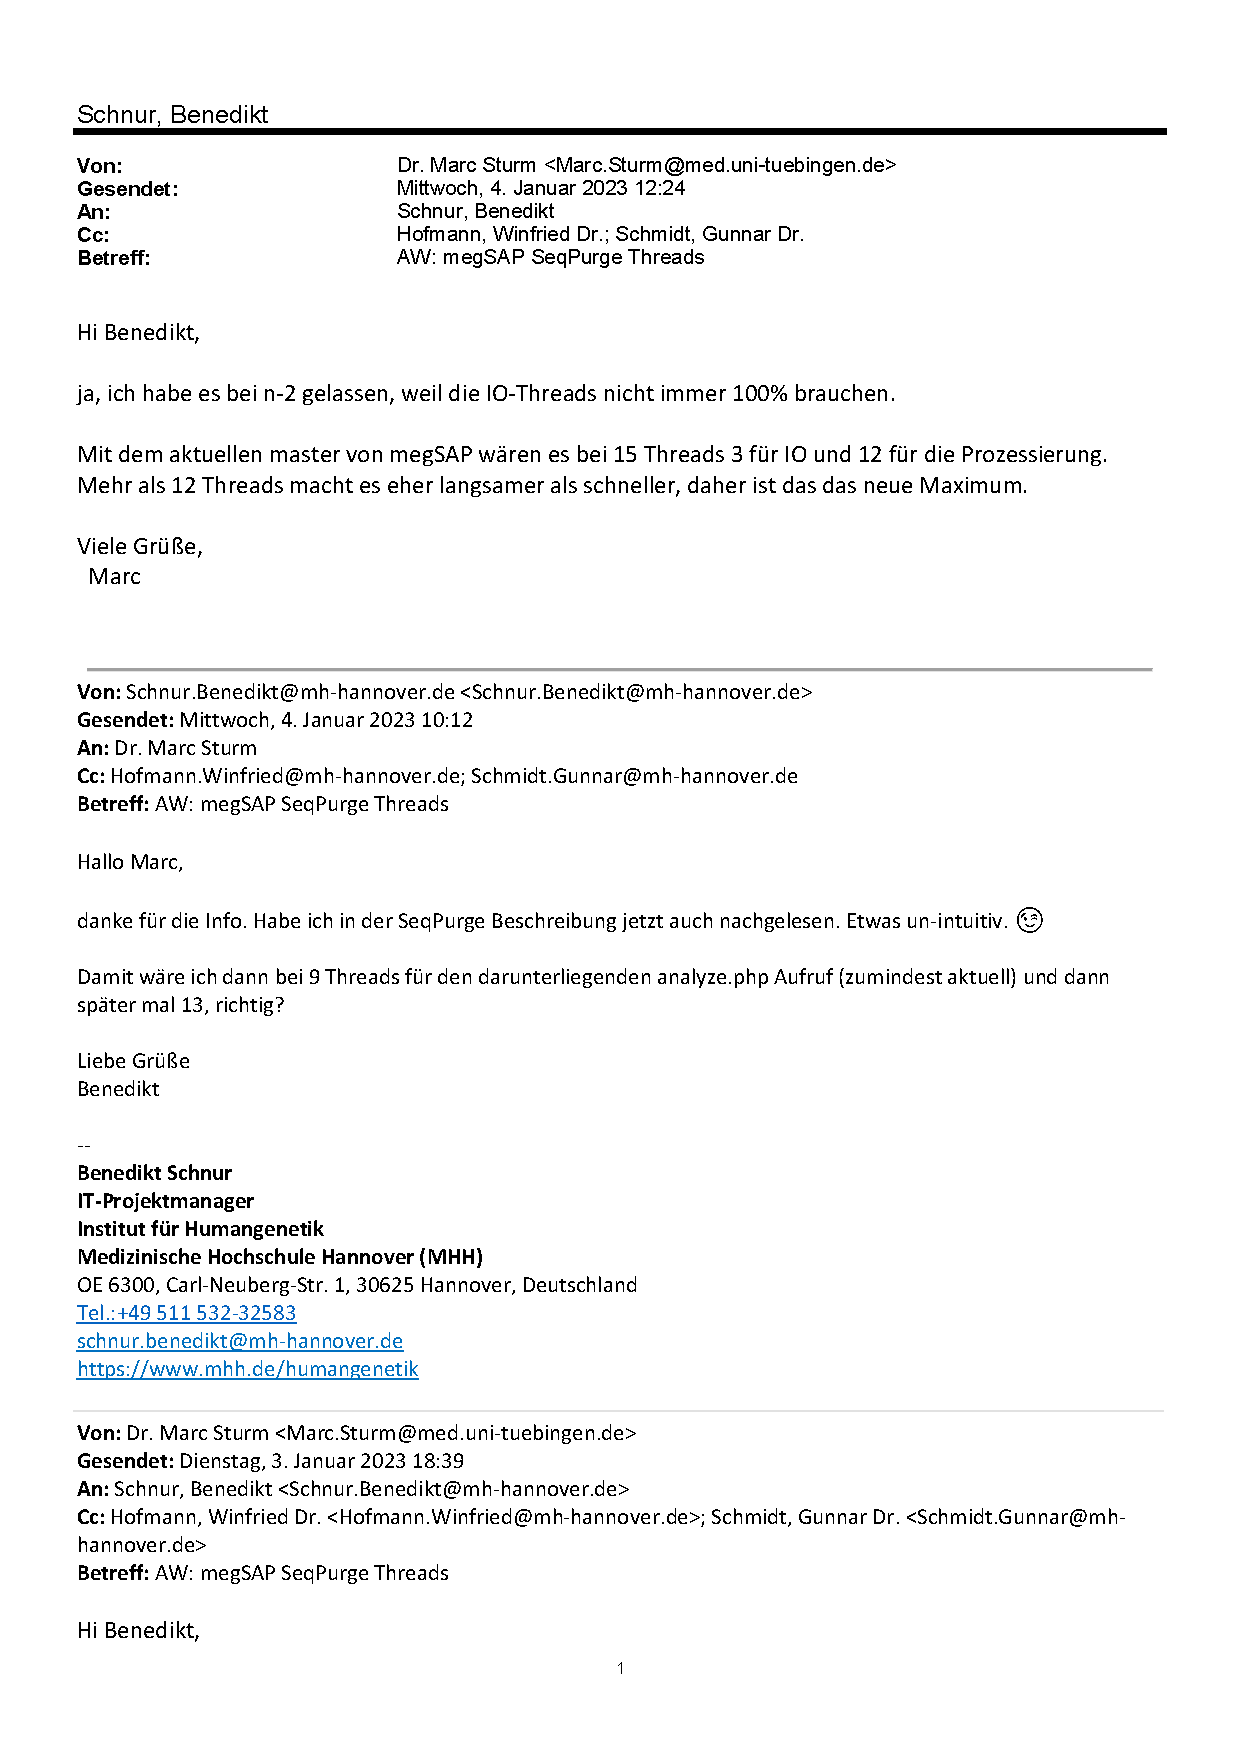
\includegraphics[width=0.9\textwidth,height=0.9\textheight,keepaspectratio,page=1]{correspondence_sturm_seqpurge}
	\caption[Correspondence with Dr. Marc Sturm discussing CPU usage of SeqPurge]{Correspondence with Dr. Marc Sturm discussing CPU usage of \textit{SeqPurge}}
	\label{fig:correspondecemarc}
\end{figure}
\begin{figure}[H]\ContinuedFloat
    \centering
	\includegraphics[width=0.9\textwidth,height=0.9\textheight,keepaspectratio,page=2]{correspondence_sturm_seqpurge}
	\caption{Correspondence with Dr. Marc Sturm discussing CPU usage of SeqPurge (cont.)}
\end{figure}

\clearpage
\subsection{Nextflow Workflow With Resilience and Monitoring}\label{appendix:megsapgermlinev1}
\lstinputlisting[caption={nextflow.config (with resilience and monitoring)}, captionpos=t, label=lst:megsapnextflowconfigv1]{listings/nextflow_v1.0.config}

\clearpage
\subsection{\ac{AWS} Prize Calculation for Optimized Nextflow Workflow}\label{appendix:awspricecalculationoptimized}
\begin{figure}[H]
    \centering
	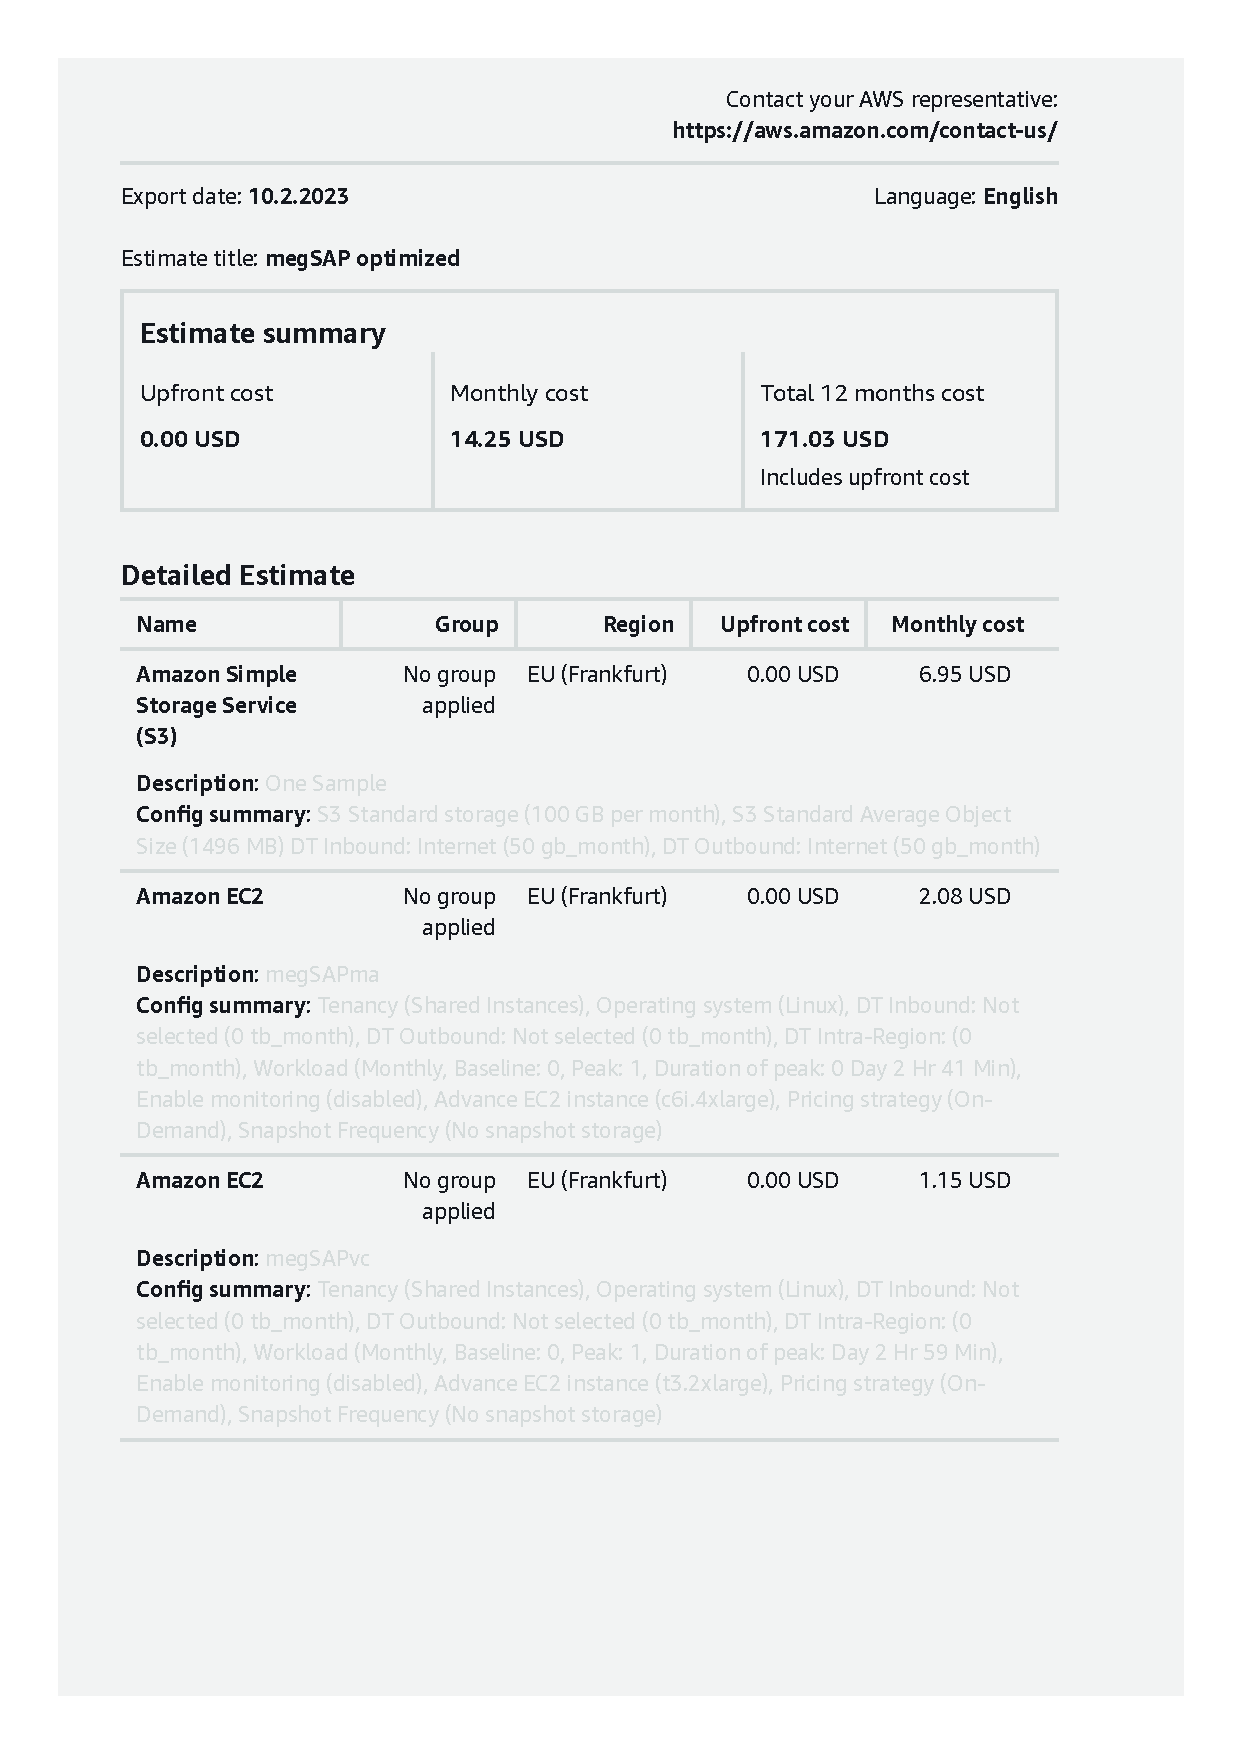
\includegraphics[width=1\textwidth,height=0.9\textheight,keepaspectratio,page=1]{AWS_Price_Calculation_One_Sample}
	\caption{\ac{AWS} prize calculation for optimized Nextflow workflow}
\end{figure}
\begin{figure}[H]\ContinuedFloat
    \centering
	\includegraphics[width=1\textwidth,height=0.9\textheight,keepaspectratio,page=2]{AWS_Price_Calculation_One_Sample}
	\caption{\ac{AWS} prize calculation for optimized Nextflow workflow (cont.)}
\end{figure}

\clearpage
\subsection{\ac{AWS} Prize Calculation for initial Nextflow Workflow}\label{appendix:awspricecalculationunoptimized}
\begin{figure}[H]
    \centering
	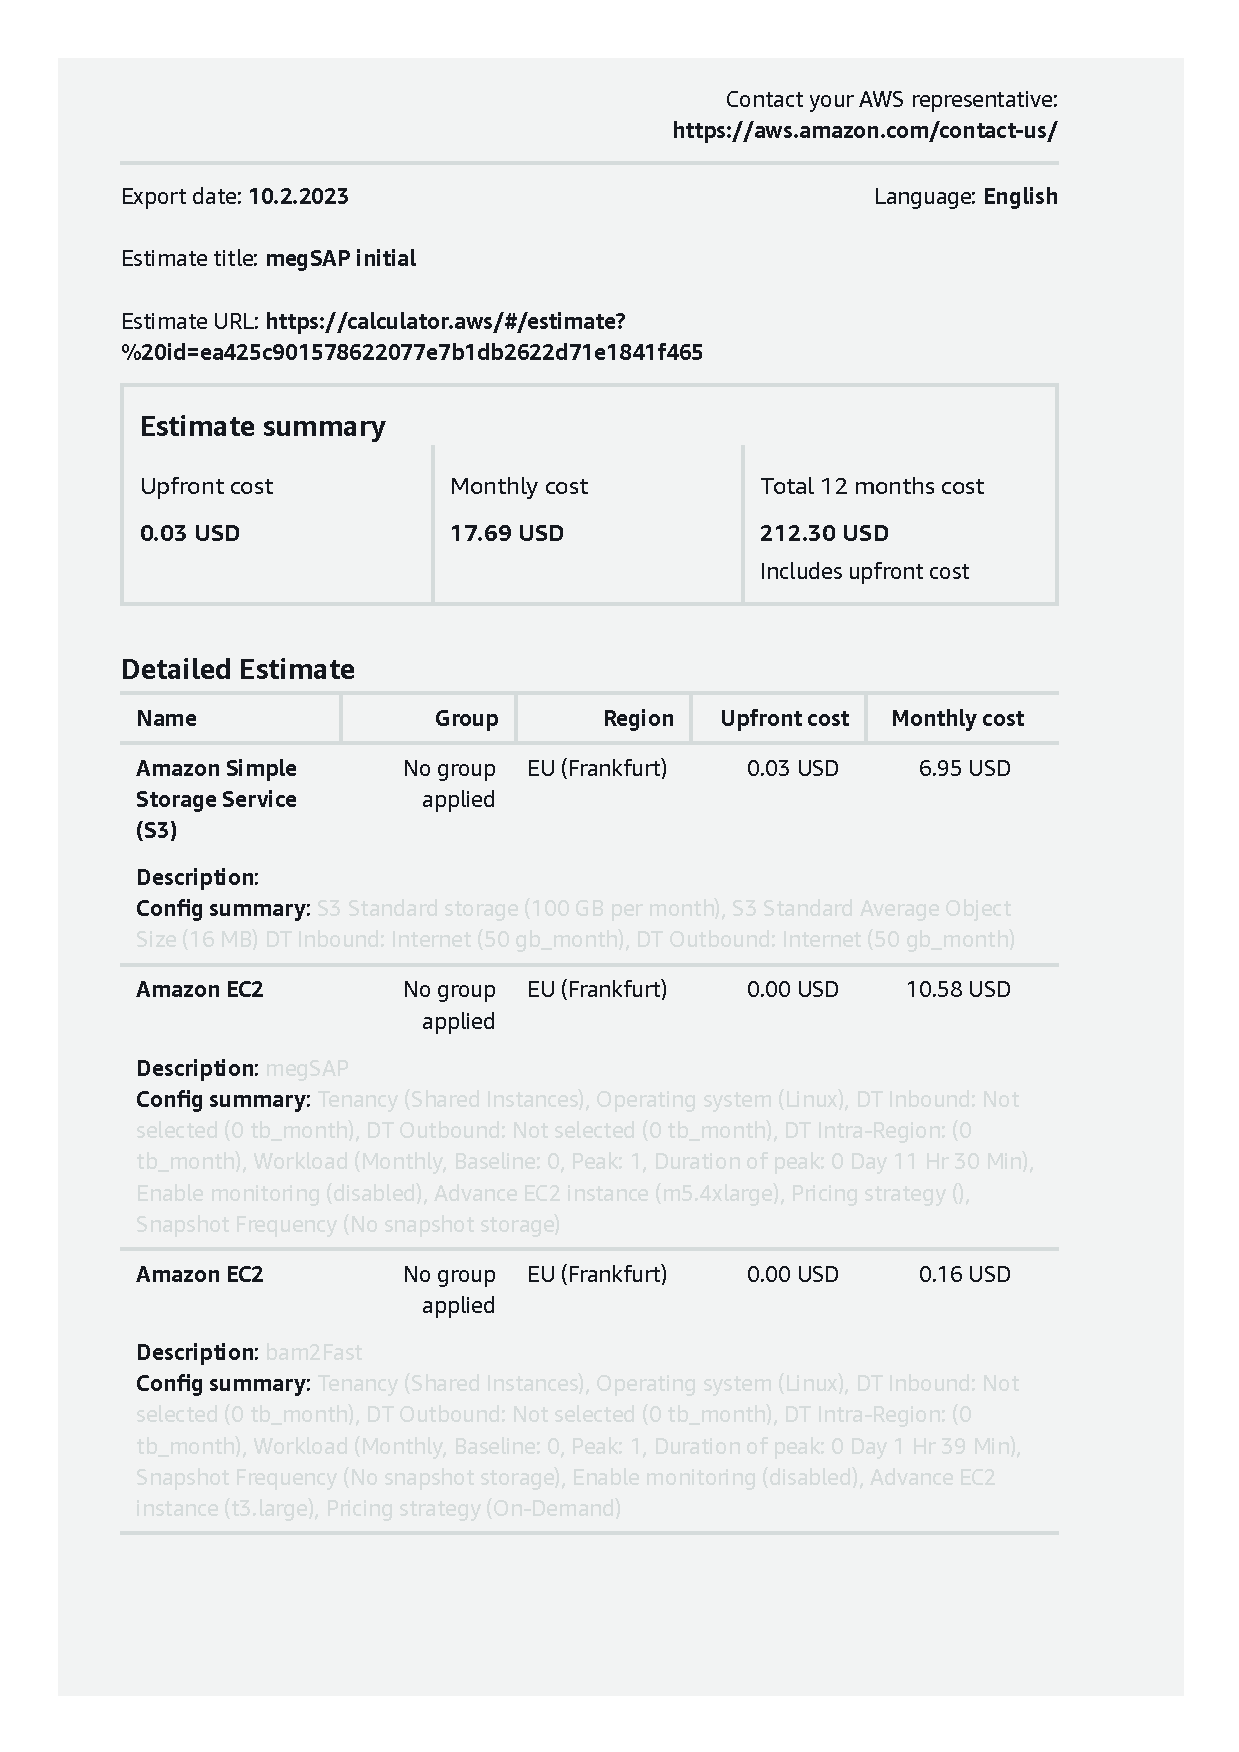
\includegraphics[width=1\textwidth,height=0.9\textheight,keepaspectratio,page=1]{AWS_Price_Calculation_One_Sample_unoptimized}
	\caption{\ac{AWS} prize calculation for initial Nextflow workflow}
\end{figure}
\begin{figure}[H]\ContinuedFloat
    \centering
	\includegraphics[width=1\textwidth,height=0.9\textheight,keepaspectratio,page=2]{AWS_Price_Calculation_One_Sample_unoptimized}
	\caption{\ac{AWS} prize calculation for initial Nextflow workflow (cont.)}
\end{figure}